\section{Exercise 1 - Implement A Benchmark Framework}
\subsection{$\sum_{i=0}^d k^i \quad \mathrm{for } \, k>0$ (Ex1.1)}
\begin{equation}
\begin{aligned}
    \sum_{i=0}^d k^i &= \sum_{i=0}^d k^i \\
    \sum_{i=0}^d k^i - k \sum_{i=0}^d k^i &= \sum_{i=0}^d k^i - k \sum_{i=0}^d k^i \\
    \sum_{i=0}^d k^i - k \sum_{i=0}^d k^i &= \sum_{i=0}^d k^i - \sum_{i=1}^{d+1} k^i \\
    \sum_{i=0}^d k^i \, (1-k) &= 1 - k^{d+1}\\
    \sum_{i=0}^d k^i   &=  \frac{k^{d+1} - 1}{k-1}
    \label{closedForm_Ex1.1}
\end{aligned}
\end{equation}

\pagebreak

\section{Exercise 2 - Implement Linear Pipeline for \texttt{MPI\_Bcast} and \texttt{MPI\_Reduce}}

Text for Ex2.
\begin{figure}[h]
    \begin{center}
        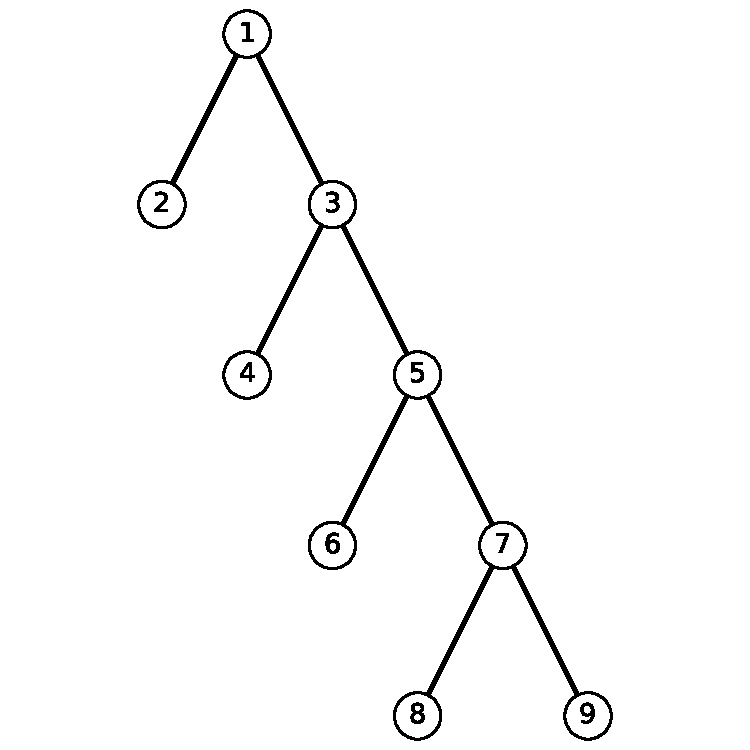
\includegraphics[width=0.3\linewidth]{figures/Ex1_2_c.pdf}
        \caption{Complete (but unbalanced) binary tree of height $d = 4$ with $p = 9$ nodes.}
    \end{center}
\end{figure}
\pagebreak


\section{Exercise 3 - Combining \texttt{MPI} Processes}
Text for Ex3.
\pagebreak

